% !TeX root =  main.tex

\chapter{Polynomial and Rational Functions}

\section{Quadratic Functions}
\begin{definition}
  A function $f(x)=ax^2+bx+c$ with $a\ne 0$ is called a \textbf{quadratic function}. Its graph is called a \textbf{parabola}. By completing the square (let $h=-\dfrac{b}{2a}$ and $k=f(h)$), a quadratic function can be written in the \textbf{standard form} (or \textbf{vertex form}): $f(x)=a(x-h)^2+k$. The vertical line $x=-\dfrac{b}{2a}$ (or $x=h$) is called the \textbf{axis of symmetry}. The \textbf{vertex} $(h,k)$ is the intersection of the axis of symmetry and the parabola.
\end{definition}
\begin{note}
  The $y$-intercept of a quadratic function is $(0, f(0))$. The $x$-coordinates of $x$-intercepts are the zeros (or roots) of the function $f$, that is, the solutions of the equation $f(x)=0$.
\end{note}

\begin{example}
  Find the vertex form of the quadratic function $f(x)=2 x^{2} + 4 x + 1$ and determine the vertex, axis of symmetry, $x$-intercepts, and $y$-intercept of the function.
\end{example}

\begin{note}
  \begin{itemize}
    \item A quadratic function $f(x)=ax^2+bx+c$ can be obtained from $y=x^2$ by a combination of vertical stretch by a factor $|a|$, a vertical reflection if $a<0$, a vertical shift of $f\left(-\frac{b}{2a}\right)$ units, and a horizontal shift of $-\frac{b}{2a}$ units.
    \item The domain of a quadratic function is $(-\infty, \infty)$.
    \item If $a>0$, then the parabola opens upward, the function has an absolute minimum $f\left(-\frac{b}{2a}\right)$, and the domain of the function is $[f\left(-\frac{b}{2a}\right), \infty)$.
    \item If $a<0$, then the parabola opens downward, the function has an absolute maximum $f\left(-\frac{b}{2a}\right)$, and the domain of the function is $(-\infty,f\left(-\frac{b}{2a}\right)]$.
  \end{itemize}
\end{note}
\newpage

\begin{example}
 Find the vertex form equation for the quadratic function $g$ in figure below as a transformation of $f(x)=x^2$, and then simplify the equation into general form.

 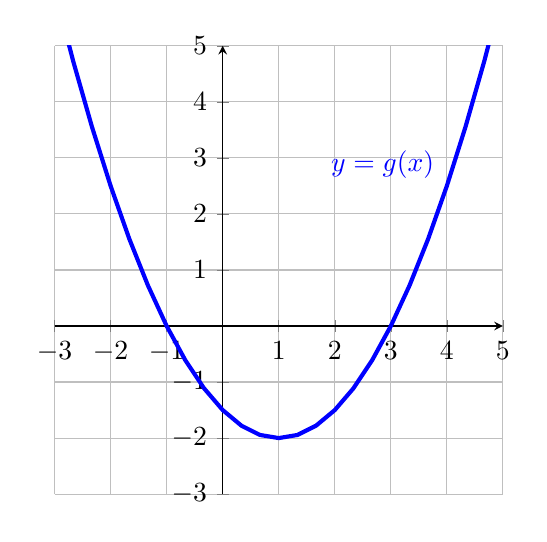
\begin{tikzpicture}
  \begin{axis}[
  axis lines=middle,
  unit vector ratio=1 1,
  ymajorgrids=true,
  xmajorgrids=true,
  xmin=-3,
  xmax=5,
  ymin=-3,
  ymax=5,
  xtick={-10,-9,...,10},
  ytick={-6,-5,...,6},]
  \addplot[blue, line width=1.5pt, domain=-3:5] {1/2*(x-1)^2-2} node[pos=0.8, above left] {$y=g(x)$};
  \end{axis}
  \end{tikzpicture}
\end{example}
\vspace*{-0.2\textheight}

\begin{example}
  Find the domain and range of each function.\\
  \begin{enumerate*}
    \item $f(x)=3x^2+6x-5$.
    \item $f(x)=-2x^2+4-1$.\hfill\null
  \end{enumerate*}
\end{example}

\begin{example}
  A backyard farmer wants to enclose a rectangular space for a new garden within her fenced backyard. She has purchased 80 feet of wire fencing to enclose three sides, and she will use a section of the backyard fence as the fourth side. What's the maximal possible area of the garden.
\end{example}

\newpage

\begin{example}
  A local newspaper currently has 84,000 subscribers at a quarterly charge of \$30. Market research has suggested that if the owners raise the price to \$32, they would lose 5,000 subscribers. Assuming that subscriptions are linearly related to the price, what price should the newspaper charge for a quarterly subscription to maximize their revenue?
\end{example}

\begin{example}
  A ball is thrown upward from the top of a 40-foot-high building at a speed of 80 feet per second. The ball's height above ground can be modeled by the equation \(H(t)=-16t^2+80t+40\).
\begin{enumerate}
  \item When does the ball reach the maximum height?
  \item What is the maximum height of the ball?  
  \item When does the ball hit the ground?
\end{enumerate}
\end{example}

\newpage

\section*{Exercise}

\begin{exercise}
  For each of the following functions,
  \begin{enumerate*}[label={(\alph*)}]
    \item $f(x)=x^2-4x+1$,
    \item $f(x)=-2x^2-4x+1$,\hfill\null
  \end{enumerate*}
  \begin{enumerate}
    \item write the function in vertex form,
    \item find the axis of symmetry,
    \item find the vertex,
    \item find the $y$-intercept,
    \item find the $x$-intercepts if they exist,
    \item find the domain and range,
    \item find the global maximum or minimum if it exists.
  \end{enumerate}
\end{exercise}

\begin{exercise}
  Find the vertex form equation for the quadratic function $f$ in figure below, and then simplify the equation into general form.
 
  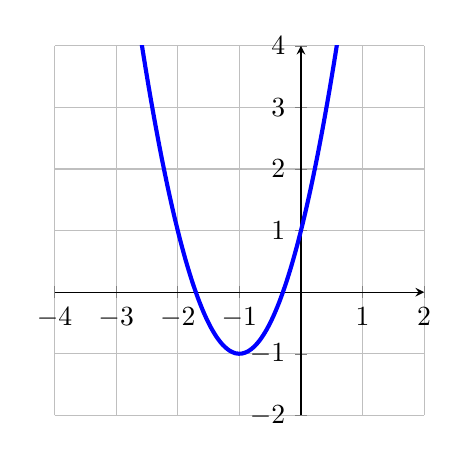
\begin{tikzpicture}
   \begin{axis}[
    width=0.6\textwidth,
   axis lines=middle,
   unit vector ratio=1 1,
   ymajorgrids=true,
   xmajorgrids=true,
   xmin=-4,
   xmax=2,
   ymin=-2,
   ymax=4,
   xtick={-10,-9,...,10},
   ytick={-6,-5,...,6},]
   \addplot[blue, line width=1.5pt, smooth,samples=100] {2*(x+1)^2-1} node[pos=0.2, right] {$y=f(x)$};
   \end{axis}
   \end{tikzpicture}
 \end{exercise}

\newpage

\begin{exercise}
  Find the dimensions of the rectangular parking lots producing the greatest area given that \(500\) feet of fencing will be used to for three sides.
\end{exercise}

\begin{exercise}
  A rocket is launched in the air. Its height, in meters above sea level, as a function of time, in seconds, is given by \(h(t)=-4.9t^2+229t+234\). Find the maximum height the rocket attains.
\end{exercise}

\begin{exercise}
  A soccer stadium holds \(62,000\) spectators. With a ticket price of \(\$11\), the average attendance has been \(26,000\). When the price dropped to \(\$9\), the average attendance rose to \(31,000\). Assuming that attendance is linearly related to ticket price, what ticket price would maximize revenue?
\end{exercise}

\newpage

\section{Power and Polynomial Functions}

\begin{definition}
  A \textbf{power function} is a function that can be represented in the form
\[f(x)=kx^p,\]
where \(k\) and \(p\) are real numbers, and \(k\) is known as the \textbf{coefficient}.
\end{definition}

\begin{example}
  Determine if the function is a power function.\\
  \begin{enumerate*}
    \item $f(x)=-2x^3$
    \item $f(x)=\dfrac{1}{x^2}$
    \item $f(x)=\sqrt[3]{x}$
    \item $f(x)=2^x$
    \item $f(x)=2x^2\cdot 3x^5$
    \item $f(x)=\dfrac{x}{x+1}$
  \end{enumerate*}
\end{example}

\begin{definition}
  The \textbf{end behavior} of a function $f$ is the general direction that the function $f$ approaches as $x$ goes to $\infty$ or $-\infty$. 
  
  We use an arrow $\to$ to describe ``goes to'' or ``approaches to''. 
  The notation $x\to \infty$ or $x\to -\infty$ means ``$x$ goes to infinity'' or ``$x$ goes to negative infinity'' respectively.
  The notation $f(x)\to \infty$ or $f(x)\to -\infty$ means ``$f(x)$ goes to infinity'' or ``$f(x)$ goes to negative infinity'' respectively.

  If $f(x)\to b$ as $x\to \infty$ or $x\to -\infty$, then we say the line $y=b$ is a \textbf{horizontal asymptote}.
\end{definition}

\begin{howto}
  To determine the end behavior of a function $f$, take a large positive number $N$. 
  
  If $f(N)$ is a large positive number, then $f(x)\to \infty$ as $x\to \infty$. 
  
  If $-f(N)$ is a large positive number, then $f(x)\to -\infty$ as $x\to \infty$.
  
  If $f(-N)$ is a large positive number, then $f(x)\to\infty$ as $x\to -\infty$. 
  
  If $-f(-N)$ is a large positive number, then $f(x)\to-\infty$ as $x\to -\infty$.
\end{howto}

\begin{example}
  Determine the end behavior(s) of the function.\\
  \begin{enumerate*}
    \item $f(x)=-2x^3$
    \item $f(x)=\dfrac{1}{x^2}$
    \item $f(x)=\sqrt[3]{x}$\hfill\null
  \end{enumerate*}
\end{example}

\newpage

\begin{definition}
  Let $n$ be a non-negative integer. A \textbf{polynomial function} of \textbf{degree} $n$ is a function that can be written in the form 
  \[f(x)=a_nx^n + \cdots + a_2x^2 + a_1x + a_0.\]
\begin{itemize}
  \item Each \(a_i\) is called a \textbf{coefficient}. 
  \item Each product \(a_ix^i\) is called a \textbf{term} of a polynomial function.
  \item The term $a_nx^n$ is called the \textbf{leading term}. The number $a_n$ is called the \textbf{leading coefficient}.
  \item The number $a_0$ is called the \textbf{constant term}.
\end{itemize}
\end{definition}

\begin{note}
  The end behavior of a polynomial function $f(x)=a_nx^2+\cdots +a_0$ of degree $n$ is completely determined by the end behavior of the power function $g(x)=a_nx^n$.
  
  The domain of a polynomial function is $(-\infty, \infty)$. The range of an odd degree polynomial function is also $(-\infty, \infty)$. The range of an even degree polynomial function is either $[y_\text{min}, \infty)$ if $a_n>0$ or $(-\infty, y_\text{max}]$ if $a_n<0$, where $y_\text{min}$ (respectively, $y_\text{max}$) is the absolute minimum (respectively, maximum) of the function. 
\end{note}

\begin{example}
  Determine the end behavior of the function.\\
  \begin{enumerate*}
    \item $f(x)=2x^4-3x+1$
    \item $g(x)=-3x^3+2x^2-x$
    \item $h(x)=-4x^6-7x^5+10x^4+2$\hfill\null
  \end{enumerate*}
\end{example}

\begin{example}
  Identify the degree, the leading therm and the end behavior of the polynomial function.\\
  \begin{enumerate*}
    \item $f(x)=-3x^2(x-1)(x+4)$
    \item $f(x)=2x^3(1-x)(x+1)$\hfill\null
  \end{enumerate*}
\end{example}

\newpage

\begin{definition}
  If $f$ is a polynomial function, then a number $c$ is called a \textbf{zero} of $f$ if $f(c)=0$.
\end{definition}

\begin{proposition}
  Let $f$ be a polynomial and $c$ a real number. Then the following are equivalent:
  \begin{enumerate}
    \item $c$ is a zero of $f$.
    \item $x=c$ is a solution of the equation $f(x)=0$.
    \item $x-c$ is a factor of $f(x)$.
    \item $(c,0)$ is an $x$-intercept of the function of $y=f(x)$.
  \end{enumerate}
\end{proposition}

\begin{example}
  Find $x$-intercepts and the $y$-intercept of the polynomial function $f(x)=x^{3} + 3 x^{2} - x - 3$.
\end{example}

\begin{example}
  Find $x$-intercepts and the $y$-intercept of the polynomial function $f(x)=x^4+2x^2-3$.
\end{example}

\begin{definition}
  A \textbf{turning point} (also known as a local extremum) is a point at which the function values change from increasing to decreasing or decreasing to increasing.
\end{definition}

\begin{theorem}[Fundamental Theorem of Algebra\footnotemark]
  A degree $n$ polynomial function has at least one complex zero.
\end{theorem}

\footnotetext{A relatively elementary proof can be found at \href{https://tinyurl.com/tFToA}{https://tinyurl.com/tFToA}.}

\begin{proposition}
  A degree $n$ polynomial function may have at most $n$ real zeros and $n-1$ turning points.
\end{proposition}

\newpage

\begin{example}
  Consider the polynomial function  $f(x)=(x-2)(x+1)(x-4)$. Determine the zeros, the number of turning points, the $x$-intercepts, and the $y$-intercept.
\end{example}


\begin{example}
  What can we conclude about the leading term of the polynomial function $y=f(x)$ represented by the graph below.\\
  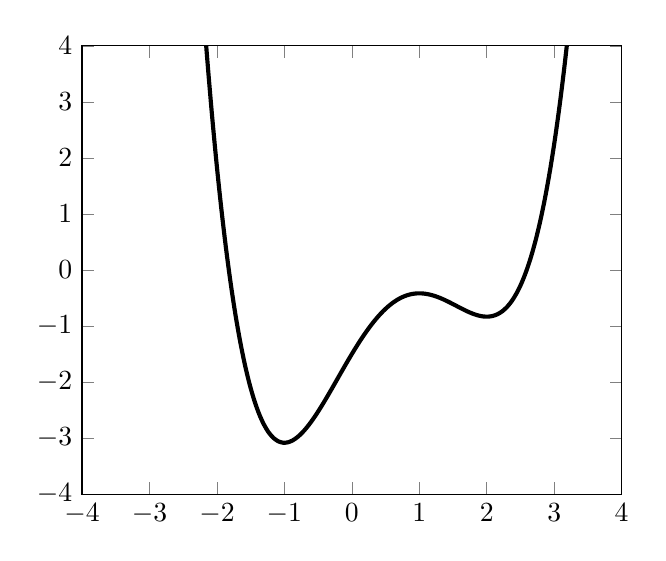
\begin{tikzpicture}
    \begin{axis}[
    xmin=-4,
    xmax=4,
    ymin=-4,
    ymax=4,
    xtick={-10,-9,...,10},
    ytick={-10,-9,...,10},]
    \addplot[line width=1.5pt, smooth, samples=100, domain=-3:4] {1/4*(x)^(4)-2/3*(x)^(3)-1/2*(x)^(2)+2*(x)-3/2} node[pos=0.9, left] {$y=f(x)$};
    \end{axis}
  \end{tikzpicture}
\end{example}
\vspace*{-0.4\textheight}


\newpage

\section*{Exercises}

\begin{exercise}
  Find the degree and leading coefficient, and determined the end behavior for the given polynomial.\\
  \begin{enumerate*}
    \item $f(x)=-2x^4$
    \item $f(x)=2x^5-x^3$
    \item $f(x)=-2x(1-x^2)$
    \item $f(x)=(x^2-1)(2x-1)(x+2)$
  \end{enumerate*}
\end{exercise}

\begin{exercise}
  Find $x$-intercepts (if they exist) and the $y$-intercept of the polynomial function.\\
  \begin{enumerate*}
  \item $f(x)=-2x^4+x^2+1$
  \item $f(x)=2x+x^3-3x^5$
  \item $f(x)=x^{3} + x^{2} - 4 x - 4$
\end{enumerate*}
\end{exercise}

\newpage
\section{Graphs of Polynomial Functions}

\begin{definition}
  We say a zero $c$ of a polynomial function $f$ has the \textbf{multiplicity} $k$ if $f(x)=(x-c)^kg(x)$ and $c$ is not a zero of $g$.
\end{definition}

\begin{example}
  Find the zeros of the polynomial function $f(x)=x^3(x-1)^2(x-2)$ and determine their multiplicities.
\end{example}

\begin{example}
  A polynomial function $P$ of degree 3 has two zeros $1$ and $2$ with multiplicity $2$ and $1$ respectively. The $y$-intercept is $(0, -4)$. Find an equation for $P$.
\end{example}


\begin{note}[Local Graph Near a Zero]
  Let $f$ be a polynomial with positive leading coefficient and $c$ is a zero of $f$ of the multiplicity $m$. The local shape of a polynomial function with positive leading coefficient near a zero is of one of the following types, or a vertical reflection of that.
  \begin{center}
    \begin{tikzpicture}
      \begin{axis}[
        title={$k=1$},
        width=0.4\textwidth,
        xmin=-1,
        xmax=1,
        ymin=-1,
        ymax=1,
        grid=none,
        xtick={0},
        extra x ticks={0},
        xticklabel={$c$},
        ylabel=\empty,
        ytick=\empty,
        y axis line style={draw=none},
      ]
      \addplot[line width=1.5pt,domain=-1:1] {-1/4*x*(x-2)*(x+2)};
      \end{axis}
    \end{tikzpicture}\hfil
    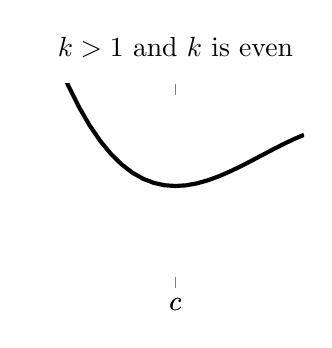
\begin{tikzpicture}
      \begin{axis}[
        title={$k>1$ and $k$ is even},
        width=0.4\textwidth,
        xmin=-1,
        xmax=1,
        ymin=-1,
        ymax=1,
        grid=none,
        xtick={0},
        extra x ticks={0},
        xticklabel={$c$},
        ylabel=\empty,
        ytick=\empty,
        y axis line style={draw=none},
      ]
      \addplot[line width=1.5pt,domain=-1:1] {-1/2*x^2*(x-2)};
      \end{axis}
    \end{tikzpicture}\hfil
    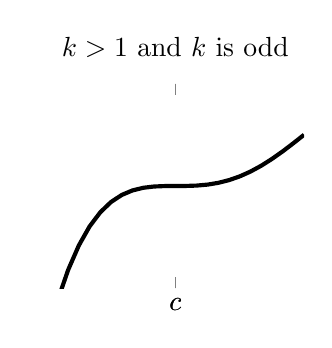
\begin{tikzpicture}
      \begin{axis}[
        title={$k>1$ and $k$ is odd},
        width=0.4\textwidth,
        xmin=-1,
        xmax=1,
        ymin=-1,
        ymax=1,
        grid=none,
        xtick={0},
        extra x ticks={0},
        xticklabel={$c$},
        ylabel=\empty,
        ytick=\empty,
        y axis line style={draw=none},
      ]
      \addplot[line width=1.5pt,domain=-1:1] {-1/2*x^3*(x-2)};
      \end{axis}
    \end{tikzpicture}
  \end{center}
\end{note}

\newpage

\begin{example}
  Use the graph of the function of degree 6 in the figure below to identify the zeros of the function and their possible multiplicities.\\
  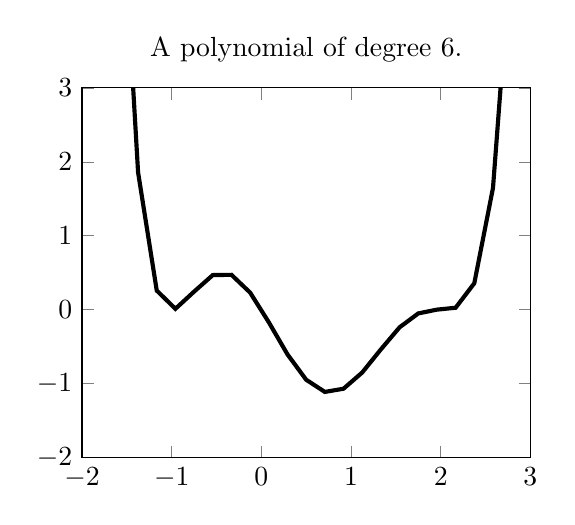
\begin{tikzpicture}
    \begin{axis}[
      width=0.6\textwidth,
      title={A polynomial of degree 6.},
      xmin=-2,
      xmax=3,
      ymin=-2,
      ymax=3,
      xtick={-3,-2,...,3},
      ytick={-3,-2,...,3}
    ]
    \addplot[line width=1.5pt, domain=-2:3] {1/4*x*(x+1)^2*(x-2)^3};
    \end{axis}
  \end{tikzpicture}
\end{example}


\begin{example}
  Find a polynomial of the least degree whose graph is given below.\\
  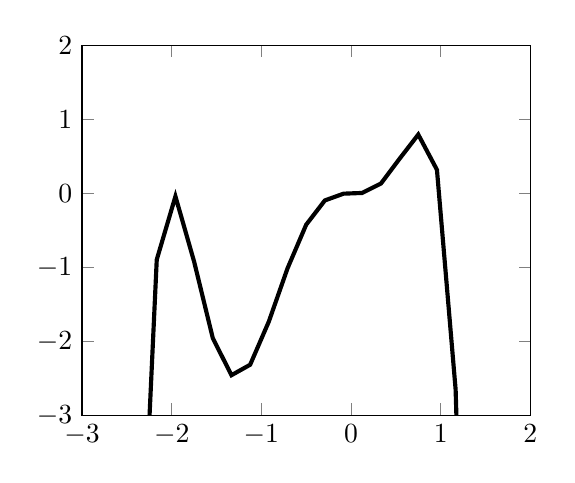
\begin{tikzpicture}
    \begin{axis}[
      width=0.6\textwidth,
      % title={A polynomial of degree 6.},
      xmin=-3,
      xmax=2,
      ymin=-3,
      ymax=2,
      xtick={-6,-5,...,3},
      ytick={-6,-5,...,3}
    ]
    \addplot[line width=1.5pt, domain=-3:2] {-(x-1)*x^3*(x+2)^2};
    \end{axis}
  \end{tikzpicture}
\end{example}

\newpage

\begin{definition}
  A \textbf{continuous} function has no breaks in its graph. A \textbf{smooth} function is a continuous function whose graph that has no sharp corners.
\end{definition}
\begin{note}
  Polynomial functions are smooth functions.
\end{note}

\begin{theorem}[Intermediate Value Theorem\footnotemark]
  If $f$ is a continuous function and $f(a)f(b)<0$, then there exists at least one value $c$ between $a$ and $b$ such that $f(c)=0$. In particular, the theorem holds true for polynomial functions. 
\end{theorem}
\footnotetext{A proof of the theorem can be found in \href{https://tinyurl.com/ivtcont}{https://tinyurl.com/ivtcont}.}
  
\begin{corollary}
  Let $f$ be a polynomial function, $a$ and $b$ real zeros of $f$. If $f$ has no other zeros between $a$ and $b$, then either $f(x)>0$ for all $x$ between $a$ and $b$ or $f(x)<0$ for all $x$ between $a$ and $b$.
\end{corollary}

\begin{theorem}[Rolle's Theorem for Polynomial Functions]
  Let $f$ be a polynomial function, $a$ and $b$ two zeros. Then $f$ has at lease one local extremum (turning point) between $a$ and $b$.
\end{theorem}
  
\begin{example}
  Determine if the polynomial function $f(x)=5x^4-2x^3-20$ has a zero on the interval $[1, 2]$.
\end{example}

\begin{howto}[Graph a Polynomial Function]
\begin{enumerate}
  \item Plot the $y$-intercept.
  \item Determine the real zeros and their multiplicities, and sketch local graph near $x$-intercepts.
  \item Determine the end behavior and sketch the graph of the left and right tails.
  \item Using symmetry to plot additional points if possible.
  \item Use test points to determine whether the graph of the polynomial lies above or below the $x$-axis over the intervals between zeros, and estimate the locations of turning points.
  \item Connect points and local graphs smoothly.
\end{enumerate}
\end{howto}

\newpage

\begin{example}
  Sketch the graph of the polynomial function $f(x)=(x-4)(x-1)^2 (x+3)$.  
\end{example}
\newpage

\section*{Exercises}

\begin{exercise}
  Find the $t$-intercepts and the $P$-intercept of the polynomial function $P(t)=3t^4-15t^3+12t^2$.
\end{exercise}

\begin{exercise}
    A polynomial function $P$ of degree 3 has two zeros $1$ and $2$ with multiplicity $2$ and $1$ respectively. The $y$-intercept is $(0, -4)$. Find an equation for $P$.
\end{exercise}

\newpage

\begin{exercise}
  Find a polynomial of the least degree whose graph is given below.\\
  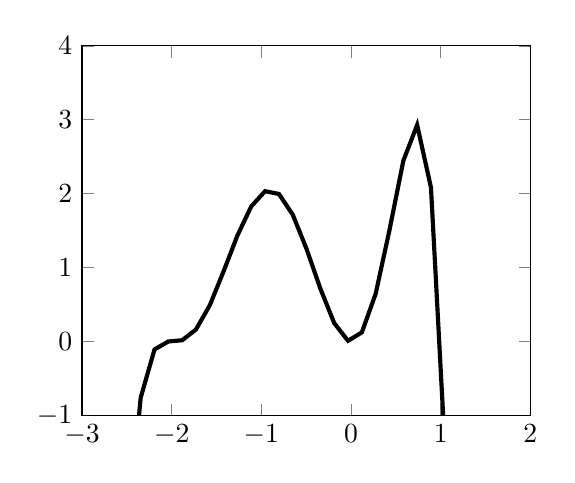
\begin{tikzpicture}
    \begin{axis}[
      width=0.6\textwidth,
      % title={A polynomial of degree 6.},
      xmin=-3,
      xmax=2,
      ymin=-1,
      ymax=4,
      xtick={-6,-5,...,6},
      ytick={-6,-5,...,6}
    ]
    \addplot[line width=1.5pt, domain=-2.5:1.2] {-(x-1)*x^2*(x+2)^3};
    \end{axis}
  \end{tikzpicture}
\end{exercise}
\vspace*{-0.2\textheight}

\begin{exercise}
  Sketch the graph of the polynomial function $f(x)=x^{4} - 2 x^{3} + x^{2}$.
\end{exercise}

\newpage
\section{Dividing of Polynomials}

\begin{theorem}[Division Algorithm]
  Let $p(x)$ and $d(x)$ be two polynomial. Suppose that \(d(x)\) is non-zero and the degree of \(d(x)\) is less than or equal to the degree of \(f(x)\). Then there exist unique polynomials \(q(x)\) and \(r(x)\) such that
  \[p(x)=d(x)q(x)+r(x)\]
and the degree of $r(x)$ is less than the degree of $d(x)$.
\end{theorem}
\begin{definition}
 In the above theorem, $p(x)$ is called the \textbf{dividend}, $d(x)$ is called the \textbf{divisor}, $q(x)$ is called the \textbf{quotient} and $r(x)$ is called the \textbf{remainder}.
 If $r(x)=0$, then we say that $d(x)$ \textbf{divides} $p(x)$.
 
 A divison algorithm\footnotemark~ is an algorithm which computes the quotient and the reminder. 

 Polynomial long division is a divison algorithm. Another shorthand division algorithm is the synthetic division. 
\end{definition}
\footnotetext{See wikipedia page on \href{https://en.wikipedia.org/wiki/Polynomial_long_division}{Polynomial long division} for various division algorithms.}

\begin{example}
  Divide \(6x^3+11x^2-31x+15\) by \(3x-2\).
\end{example}

\begin{example}
  Divide \(4x^4+3x^2-1x+5\) by \(2x^2-x+3\).
\end{example}

\newpage
\begin{definition}
  Synthetic division is a shortcut that can be used when the divisor is linear binomial in the form $x-c$. In synthetic division, only the coefficients are used in the division process.
\end{definition}

\begin{example}
  Use synthetic division to divide $4x^3+10x^2-6x-20$ by $x+2$.
\end{example}

\begin{example}
  Use synthetic division to divide $-9x^4+10x^3+7x^2-6$ by $x-1$.
\end{example}

\newpage
\section*{Exercises}

  \begin{exercise}
    Divide $3x^2 - 7 x - 3$ by $3x-1$.
  \end{exercise}

  \begin{exercise}
    Divide $16 x^3 - 12 x^2 + 20 x - 3$ by $4x+5$.
  \end{exercise}

  \begin{exercise}
  Use synthetic division to divide $5x^2-3x-36$ by $x-3$.
  \end{exercise}

  \begin{exercise}
  Divide $2 x^4 + 4 x^3 - 3 x^2 - 5 x - 2$ by $x+2$.
  \end{exercise}

\newpage
\section{Zeros of Polynomials}

\begin{theorem}[The Remainder Theorem]
If a polynomial $f(x)$ is divided by $x-c$, then the remainder is the value $f(c)$.
\end{theorem}
\begin{example}
  Use the Remainder Theorem to evaluate $f(x)=6x^4-x^3-15x^2+2x-7$ at $x=2$.
\end{example}

\begin{theorem}[The Rational Zero Theorem]
Let $f(x)=a_nx^n+a_{n-1}x^{n-1}+\cdots +a_1x+a_0$ be polynomial with integer coefficients. Then every rational zero of $f(x)$ is in the form $\frac{p}{q}$, where $p$ is a factor of the constant term $a_0$ and $q$ is a factor of the leading coefficient $a_n$.
\end{theorem}
\begin{example}
  List all possible rational zeros of $f(x)=2x^4-5x^3+x^2-4$.
\end{example}

\begin{example}
  Find the zeros of $f(x)=4x^3-3x-1$.
\end{example}

\newpage

\begin{theorem}[Linear Factorization Theorem]
  Let $f(x)$ be a polynomial with the degree $n>1$ and the leading coefficient $a_n$. Then
  \[f(x)=a_n(x-c_1)(x-c_2)\cdots(x-c_n),\]
  where $c_i$ are complex numbers.
\end{theorem}

\begin{theorem}[Complex Conjugation Theorem]
  Let $f(x)$ be a polynomial. If $x-(a+b~i)$ is a factor of $f$, then $x-(a-b~i)$ is also a factor of $f$. 
\end{theorem}

\begin{example}
  Find a fourth degree polynomial with real coefficients that has zeros of $-3$, $2$, $i$, such that $f(-2)=100$.
\end{example}

\begin{theorem}[Descartes' Rule of Signs\footnotemark]
  Let $f(x)=a_nx^n+a_{n-1}x^{n-1}+\cdots+a_1x+a_0$ be a polynomial function with real coefficients.

  \begin{itemize}
    \item The number of positive real zeros counted with multiplicity is either equal to the number of sign changes of $f(x)$ or is less than the number of sign changes by an even integer.
    \item The number of negative real zeros counted with multiplicity is either equal to the number of sign changes of $f(-x)$ or is less than the number of sign changes by an even integer.
  \end{itemize}
\end{theorem}
\footnotetext{For a proof, see the blogpost \href{http://math1210blog.robertborgersen.info/2012/05/proof-of-descartes-rule-of-signs/}{Proof of Descartes' Rule of Signs}}

\begin{example}
  Use Descartes' Rule of Signs to determine the possible numbers of positive and negative real zeros for $f(x)=-x^4-3x^3+6x^2-4x-12$.
\end{example}

\newpage
\section*{Exercises}

\begin{exercise}
  Find all zeros of $f(x)=2x^3+5x^2-11x+4$.
\end{exercise}

\begin{exercise}
  Find all zeros of $f(x)=x^4 + 3 x^3 + 2 x^2 - 2 x - 4$.
\end{exercise}


\begin{exercise}
  Find a fourth degree polynomial with real coefficients that has zeros of $-1$, $2$, $1+i$, such that $f(-2)=10$.
\end{exercise}

\newpage

\section{Rational Functions}
\begin{definition}
  Let $p(x)$ and $q(x)$ be polynomials with $\deg(q(x))>0$. The function $f(x)=\dfrac{p(x)}{q(x)}$ is called a rational function. The domain of $f$ is $\{x\mid q(x)\ne 0\}$.
\end{definition}

\begin{example}
  Find the domain of $f(x)=\dfrac{x+3}{x^2-9}$.
\end{example}

\begin{definition}[Vertical Asymptote]
  A \textbf{vertical asymptote} of a function $f$ is a vertical line $x=a$ where the graph of $f$ goes to positive or negative infinity as $x$ approached $a$ from left or right, that is, as $x\rightarrow a^- ~\text{or}~ a^+$, $f(x)\rightarrow \infty$, or as $x\rightarrow a^- ~\text{or}~ a^+$, $f(x)\rightarrow -\infty$, where $x\to a^-$ (or $a^+$) means $x$ approaches $a$ from the left (respectively, right).

  We say a function $f$ has a \textbf{removable discontinuities} (or \textbf{hole}) at $x=a$ if $f(x)\to b$ as $x\to a$ but $f(a)$ is undefined.
\end{definition}

\begin{proposition}
  Let $f=\dfrac{p(x)}{q(x)}$ be a rational function. If $p(a)=q(a)=0$, then $f$ has a hole at $a$. If $q(a)=0$ but $p(a)\ne 0$, then $f$ has a vertical asymptote $x=a$.
\end{proposition}

\begin{definition}[Horizontal Asymptote]
A \textbf{horizontal asymptote} of a function $f$ is a horizontal line $y=b$ where the graph of $f$ approaches to $b$ as $x$ goes to positive or negative infinity, that is,   
as $x\rightarrow \infty$, or $x\rightarrow -\infty$, $f(x)\rightarrow b$.
\end{definition}

\begin{definition}[Slanted Asysmptote]
  A \textbf{slanted asymptote} of a function $f$ is a line $y=mx+b$ with $m\ne 0$ where the graph of $f$ approaches to $mx+b$ as $x$ goes to positive or negative infinity, that is,   
as $x\rightarrow \infty$ or $x\rightarrow -\infty$, $f(x)\rightarrow mx+b$.
\end{definition}

\begin{note}
  For a rational function $f$, as $x\rightarrow \infty$ or $-\infty$, $f(x)$ approaches the asymptote only from one side of the line. This information will be helpful when sketching a graph.
\end{note}


\begin{proposition}
Let $f(x)=\dfrac{p(x)}{q(x)}=\dfrac{a_mx^m+a_{m-1}x^{m-1}+...+a_1x+a_0}{b_nx^n+b_{n-1}x^{n-1}+...+b_1x+b_0}$ be a rational function.
\begin{itemize}
  \item if $m<n$, then $f$ has a horizontal asymptote $x=0$;
  \item if $m=n$, then $f$ has a horizontal asymptote $x=\frac{a_m}{b_n}$;
  \item if $m=n+1$, then $f$ has a slated asysmptote $y=mx+b$, where $mx+b$ is the quotient of $\frac{p(x)}{q(x)}$.
  \item if $m>n+1$, then $f$ has no horizontal or slated asymptote;
\end{itemize}
\end{proposition}

\newpage

\begin{example}
  Use arrow notation to describe asymptotes of the function $f$ graphed in the figure.\\
  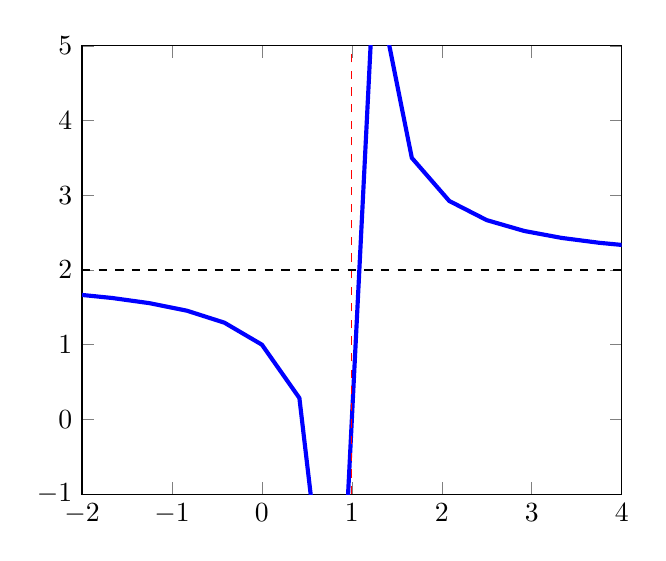
\begin{tikzpicture}
    \begin{axis}[
    xmin=-2,
    xmax=4,
    ymin=-1,
    ymax=5,
    xtick={-5,-4,...,6},
    ytick={-1,0,...,5},
    grid=none]
    \addplot[line width=1.5pt, restrict y to domain=-5:10, blue] {1/(x-1)+2} node[pos=0.8, above right] {$f$};
    \addplot+[dashed,mark=none] coordinates{(1,-1)(1,5)};
    \addplot[dashed, domain=-2:4] {2};
    \end{axis}
    \end{tikzpicture}
\end{example}
\vspace*{-0.2\textheight}
\begin{example}
  Use arrow notation to describe the slanted asymptote of the function $f$ graphed in the figure.\\
  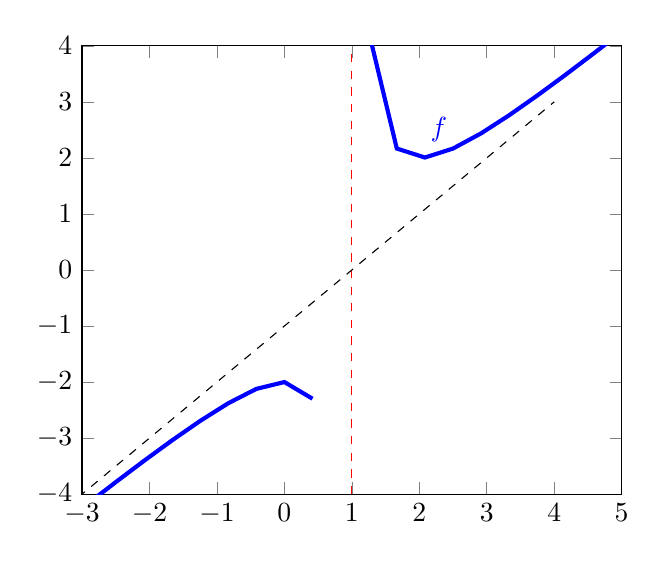
\begin{tikzpicture}
    \begin{axis}[
    xmin=-3,
    xmax=5,
    ymin=-4,
    ymax=4,
    xtick={-5,-4,...,6},
    ytick={-4,-3,...,5},
    grid=none]
    \addplot[line width=1.5pt, restrict y to domain=-5:5, blue] {1/(x-1)+x-1} node[pos=0.7, above] {$f$};
    \addplot+[dashed,mark=none] coordinates{(1,-4)(1,4)};
    \addplot[dashed,domain=-4:4] {x-1};
    \end{axis}
    \end{tikzpicture}
\end{example}
\vspace*{-0.2\textheight}

\begin{example}
Find the asymptotes of the rational function $f(x)=\dfrac{x^2+1}{2x^2-3x+1}$ if they exist.
\end{example}

\newpage

\begin{example}
Find the asymptotes of the rational function $f(x)=\dfrac{- x^{2} + 3 x - 1}{x - 1}$ if they exist.
\end{example}

\begin{example}
  Find the asymptotes and holes of the function
$f(x)=\dfrac{x^{2} + x - 6}{x^{3} - 2 x^{2} - x + 2}$ if they exist.
\end{example}

\newpage

\begin{howto}[Graph of a Rational Function]
  \begin{enumerate}
  \item Find the $y$-intercept and plot it.
  \item Find the $x$-intercept(s) and plot them.
  \item Find all vertical asymptotes and graph them as dashed lines.
  \item Find the horizontal asymptote or the slant asymptote (or neither), and graph the asymptote as a dashed line.
  \item Plot a test point in each interval whose boundary values are zeros of the denominators or the function to determine if the graph is above the axis or below the axis over that interval.
  \item Sketch the function based on the information found above.
  \end{enumerate}
\end{howto}

\begin{example}
  Sketch a graph of  $f(x)=\dfrac{(x+2)(x-3)}{(x+1)^2(x-2)}$.
\end{example}

\newpage

\section*{Exercises}

\begin{example}
  Find asymptotes of the rational function $f(x)=\dfrac{3x^2-1}{x^2+4x-5}$
\end{example}

\begin{exercise}
  Find asymptotes of the rational function $f(x)=\dfrac{x^{2}}{x + 1}$.
\end{exercise}

\begin{exercise}
  Find asymptotes and holes of the rational function $f(x)=\dfrac{(x-1)(x-2)}{x^2-4}$.
\end{exercise}
\newpage

\begin{exercise}
  Sketch a graph of the rational function $f(x)=\dfrac{(x+2)^2(x-1)}{(x+1)^2(x-2)}$.
\end{exercise}

\begin{exercise}
  Sketch a graph of the rational function  $f(x)=\dfrac{4(x+2)(x-3)^3}{(x+1)(x-2)^2}$.
\end{exercise}

\newpage
\section{Polynomial and Rational Inequalities}
\begin{howto}[Polynomial or Rational Inequalities]
\begin{enumerate}
  \item Rewrite the inequality into the form $f(x)\text{~inequality symbol~} 0$.
  \item Find all real zeros of $f(x)$.
  \item Break the \textbf{\uppercase{domain of the function}} (the whole number line if $f$ is a polynomial) into intervals using zeros from the previous step.
  \item Choose a test point from each interval to determine the sign of $f$.
  \item Determine the solutions (union of intervals in which the test point satisfies the inequality) and whether the boundary values of the intervals should be included.
\end{enumerate}
\end{howto}

\begin{example}
  Solve the inequality $x^{2} \le 7 x - 6$.
\end{example}

\begin{example}
  Solve the inequality $2 x^{3} - 3 x^{2} >  3 x - 2$.
\end{example}

\newpage

\begin{example}
  Solve the inequality $\dfrac{4-x}{x - 1}< 2$.
\end{example}

\begin{example}
  Solve the inequality $\dfrac{6 x}{(x + 1) (x + 2)}\ge 1$.
\end{example}


\newpage
\section*{Exercises}

\begin{exercise}
  Solve the inequality $-x^2>5x-6$.
\end{exercise}

\begin{exercise}
  Solve the inequality $2 x^{3} + x^{2} \le 2 x + 1$.
\end{exercise}

\newpage

\begin{exercise}
  Solve the inequality $1\ge \dfrac{x-1}{2x+1}$.
\end{exercise}

\begin{exercise}
  Solve the inequality $\dfrac{x+8}{x^2-4}<1$.
\end{exercise}
